\documentclass[a4paper]{article}

\usepackage{fontspec,xltxtra,xunicode}
\usepackage{xeCJK}
\usepackage{titlesec}
\usepackage{titletoc}
\usepackage{xcolor}
\usepackage{float}
\usepackage{pdfpages}

\title{\emph{Statistical Analysis with Missing Data}\ \ Problem 1.6\\Bootstrap,Jackknife}
\author{16212799,何浩勋}
\date{September 7, 2017}

\setCJKfamilyfont{yahei}{微软雅黑}
\newcommand{\yahei}{\CJKfamily{yahei}}

\begin{document}

\fontsize{12pt}{18pt}\selectfont\yahei
\maketitle

\section{Problem 1.6}
\paragraph{\fontsize{12pt}{16pt}\selectfont\yahei
100 trivariate normal observations
$\{(y_{i1},y_{i2},u_i),i=1,...,100\}$ on
$(Y_1, Y_2, U)$ as follows:
}

\begin{equation}
\begin{array}{lll}
y_{i1}=1+z_{i1} \\
y_{i2}=2*z_{i1}+z_{i2}\\
u_i=a*(y_{i1} - 1)+b*(y_{i2}-5)+z_{i3}
\end{array}
\end{equation}

\paragraph{\fontsize{12pt}{16pt}\selectfont\yahei
where $\{(z_{i1},z_{i2}, z_{i3}), i=1,...,100\}$ are independent standard normal deviates.
The latent variable U determines missingness of $Y_2$ as follows:}

\begin{equation}
y_{i2}\ is\ missing\ if\ u_i\ <\ 0
\end{equation}

\paragraph{\fontsize{12pt}{16pt}\selectfont\yahei
Label Description\\
origin\ : original generated Data\\
obs\ : $Y_1$ and $Y_2$ both observed\\
mis\ : $Y_1$ observed and $Y_2$ missing
}

\newpage

\paragraph{\fontsize{12pt}{16pt}\selectfont\yahei
Case 1: a=0,b=0\\
Y1(origin) : mean =8.882104e-01, std=9.724232e-01\\
Y1(obs)    : mean =9.310380e-01, std=9.661219e-01\\
Y1(mis)    : mean =8.265806e-01, std=9.781347e-01\\
origin Vs mis : t =3.3875e-01, pvalue =7.3531e-01\\
obs Vs mis    : t =5.2375e-01, pvalue =6.0164e-01\\
Conclusion : There is no Significant differences.\\
$f(M|Y_1,Y_2,U)=F(M|Z_3)$,$Z_3$ is independent of $Y_2$,$Y_1$.\\
The machenism is MCAR.
}

\begin{figure}[H]
	\centering
	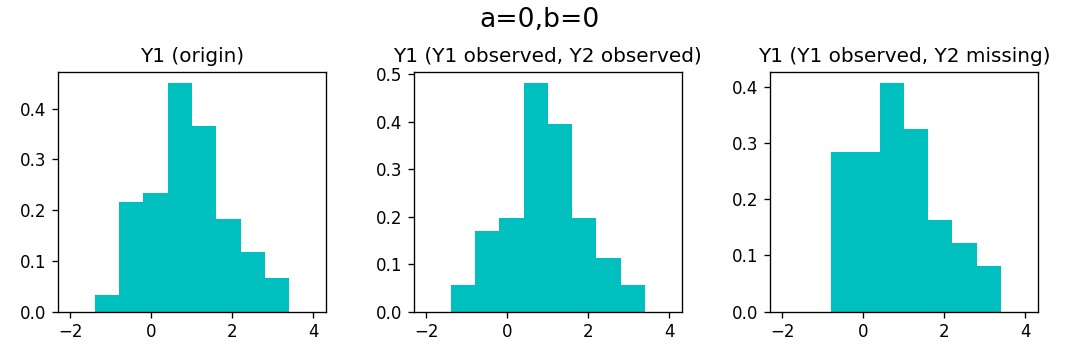
\includegraphics[scale=0.5]{a0b0.png}
	\label{pic1}
\end{figure}

\paragraph{\fontsize{12pt}{16pt}\selectfont\yahei
Case 2: a=2,b=0\\
Y1(origin) : mean =8.882104e-01, std=9.724232e-01\\
Y1(obs) : mean =1.635554e+00, std=6.775540e-01\\
Y1(mis) : mean =1.701749e-01, std=6.007170e-01\\
origin  Vs mis : t =4.7925e+00, pvalue =3.9468e-06\\
obs Vs mis : t =1.1339e+01, pvalue =1.5452e-19\\
Conclusion : There is a significant difference.\\
f(M|Y1,Y2,U) = F(M|Y1,Z3),The machenism is MAR.
}

\begin{figure}[H]
	\centering
	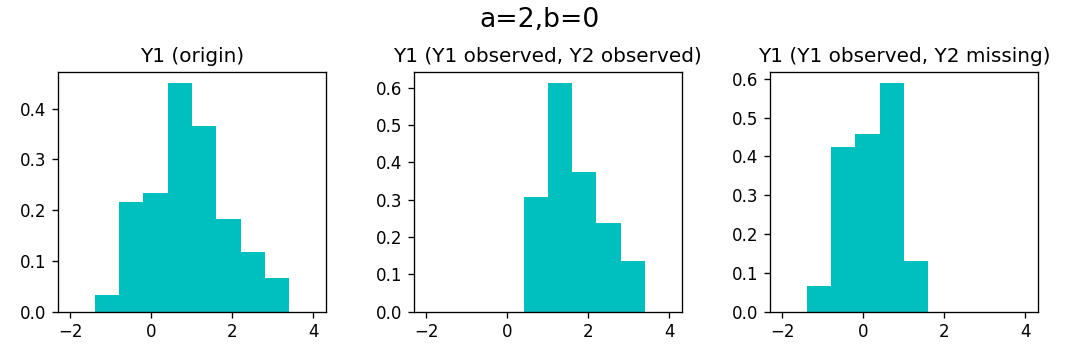
\includegraphics[scale=0.5]{a2b0.png}
	\label{pic2}
\end{figure}

\paragraph{\fontsize{12pt}{16pt}\selectfont\yahei
Case 3: a=0,b=2\\
Y1(origin) : mean =8.882104e-01, std=9.724232e-01\\
Y1(obs) : mean =1.701187e+00, std=6.813406e-01\\
Y1(mis) : mean =2.749121e-01, std=6.588037e-01\\
origin Vs mis : t =4.2122e+00, pvalue =4.2763e-05\\
obs Vs mis : t =1.0455e+01, pvalue =1.2476e-17\\
Conclusion : There is a significant difference.\\
f(M|Y1,Y2,U) = F(M|Y2,Z3),the machanism is NMAR.
}

\begin{figure}[H]
	\centering
	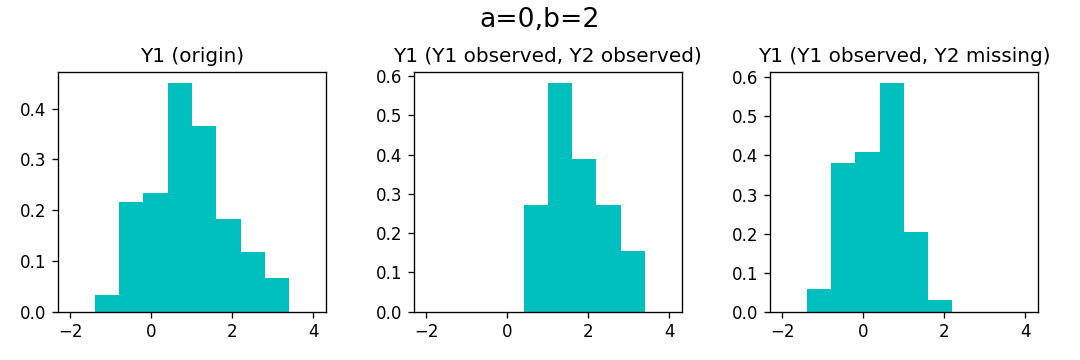
\includegraphics[scale=0.5]{a0b2.png}
	\label{pic3}
\end{figure}

\newpage
\section{Bootstrap,Jackknife}

\paragraph{\fontsize{12pt}{16pt}\selectfont\yahei
$\{X_i, i=1,...,100\}$ is a random sample from a $N(7,4)$ population.
Three methods(Moment,Bootstrap,Jackknife) are applied to estimate the population mean $\mu$ and variance $\sigma^2$.
}
\paragraph{\fontsize{12pt}{16pt}\selectfont\yahei
It appears that the traditional moment method makes the best estimation of both $\mu$ and $\sigma^2$ while another two methods also make similar estimates.Overall,There is no significant difference among the estimates made by these three methods.}

\begin{table}[h]
\fontsize{12pt}{18pt}\selectfont\yahei
\centering
	\begin{tabular}{|l|c|c|c|c|}\hline
		Method & $\mu$(estimate) & variance \\
		\hline
		Moment & 7.11961603 & 0.04063306 \\
		Bootstrap & 7.11606507 & 0.04967192\\
		Jackknife & 7.11961603 & 0.04104350\\
		\hline
	\end{tabular}
	\caption{estimates of $\mu$}
\end{table}

\begin{table}[h]
\fontsize{12pt}{18pt}\selectfont\yahei
\centering
	\begin{tabular}{|l|c|c|c|c|}\hline
		Method & $\sigma^2$(estimate) & variance\\
		\hline
		Moment & 4.06330648 & 0.26774111\\
		Bootstrap & 4.06615074 & 0.32251543\\
		Jackknife & 4.10434998 & 0.27593671\\
		\hline
	\end{tabular}
	\caption{estimates of $\sigma^2$}
\end{table}

\end{document}